\documentclass{article}

%-------------------------------------------------

%\linespread{2.0}

\usepackage{fullpage}

\usepackage{graphicx}

\usepackage{amsmath}
\usepackage{amssymb}
\usepackage{amsfonts}

\usepackage{color}

\usepackage{verbatim}

\usepackage{tikz}
\usetikzlibrary{arrows,automata}

%-------------------------------------------------

\newcommand{\FIXME}[1]{\textcolor{red}{\textbf{#1}}}

%-------------------------------------------------

\newcommand{\stdin}{\texttt{stdin}}
\newcommand{\stdout}{\texttt{stdout}}
\newcommand{\stderr}{\texttt{stderr}}

\newcommand{\PID}{\texttt{PID}}

\newcommand{\multiprocessing}{\texttt{multiprocessing}}
\newcommand{\multiprocessingConnection}{\texttt{multiprocessing.Connection}}

\newcommand{\GraceDB}{\texttt{GraceDB}}
\newcommand{\alert}{\texttt{lvalert}}

\newcommand{\lvalertListen}{\texttt{lvalert\_listen}}
\newcommand{\lvalertSend}{\texttt{lvalert\_send}}

\newcommand{\lvalertMP}{\texttt{lvalertMP}}
\newcommand{\lvalertListenMP}{\texttt{lvalert\_listenMP}}
\newcommand{\lvalertCommandMP}{\texttt{lvalert\_commandMP}}

\newcommand{\interactiveQueue}{\texttt{interactiveQueue}}
\newcommand{\parseAlert}{\texttt{parseAlert}}

\newcommand{\SortedQueue}{\texttt{SortedQueue}}
\newcommand{\QueueItem}{\texttt{QueueItem}}
\newcommand{\Task}{\texttt{Task}}

\newcommand{\lvalertMPini}{\texttt{lvalert\_listenMP.ini}}
\newcommand{\childConfigini}{\texttt{childConfig.ini}}

\newcommand{\approvalProcessor}{\texttt{approval\_processor}}
\newcommand{\eventSupervisor}{\texttt{event\_supervisor}}

\newcommand{\pythonint}{\texttt{int}}
\newcommand{\pythonfloat}{\texttt{float}}
\newcommand{\pythonstr}{\texttt{str}}
\newcommand{\pythonbool}{\texttt{bool}}
\newcommand{\pythonlist}{\texttt{list}}
\newcommand{\pythondict}{\texttt{dict}}

\newcommand{\json}{\texttt{json}}

%-------------------------------------------------
\begin{document}
%-------------------------------------------------

\title{
\lvalertMP~User's Guide
}

\author{
Reed Essick \\
reed.essick@ligo.org
}

\maketitle

\newpage

%------------------------

\tableofcontents
\listoffigures

\newpage

%------------------------

\section{introduction}

\lvalertListen~provides an extremely flexible infrastructure from which processes can listen and respond to events within \GraceDB. 
However, it currently only communicates with the forked process once (via \stdin) and therefore cannot send multiple \alert~messages to any procesess.
For most follow-up, this is not an issue.
Many processes simply respond to any new event which passes a basic FAR threshold. 
However, a few key processes will benefit from receiving all alerts about a set of events.
Indeed, passing all \alert~messages to a single process obviates the inter-process communication and associated race conditions that would be required of multiple independent processes, each forked with a separate, single \alert~message.

This guide describes how \lvalertListenMP~addresses and resolves this problem. 
In particular, we focus on a pedagogical description of the classes and methods used within the executables.
We also focus on the user's interface with the tools from the command line.

Briefly, \lvalertListenMP~uses the same interface with the \alert~servers as \lvalertListen~but forks child processes via Pythons \multiprocessing~module.
In this way, \lvalertListenMP~can communciate with the child processes repeatedly (through a shared \multiprocessingConnection~object).
The module provides a standardized way to schedule and execute follow-up activities.
While the actual follow-up implemented here is basic, it is easily extended to achieve more complicated goals.
An example is the \eventSupervisor~library.

This guide is organized as follows. In \S\ref{sec: classes, methods, configs and executables}, we enumerate and describe the basic objects, methods, configuration files, and executables defined within this module. 
This includes examples for how these might be used.
In \S\ref{sec: workflow}, we demonstrate the workflow within \lvalertListenMP~and describe how the various parts fit together to manage follow-up tasks.
Finally, we discuss existing and suggested extensions in \S\ref{sec: suggested extensions}.

%------------------------

\section{classes, methods, configs and executables}
\label{sec: classes, methods, configs and executables}

This section defines the classes (\S\ref{sec: classes}), methods (\S\ref{sec: methods}), configuration files (\S\ref{sec: configs}), and executables (\S\ref{sec: executables}) that are necessary for \lvalertListenMP~to function. 
Their interactions are described in \S\ref{sec: workflow}, so we focus on the particular responsibilities associated with each element here.

%-----------

\subsection{classes}
\label{sec: classes}

There are three (3) main classes defined within \lvalertMP:
\begin{itemize}
    \item{\SortedQueue (\S\ref{sec: SortedQueue})}
    \item{\QueueItem (\S\ref{sec: QueueItem})}
    \item{\Task (\S\ref{sec: Task})}
\end{itemize}
These objects are what allow \lvalertListenMP~to define and schedule multiple follow-up activities based on \alert~messages about multiple events within a single process.
In particular, individual activities are encapsulated as \Task objects.
Each \QueueItem~is associated with one or more \Task~objects.
\SortedQueue~contains an ordered list of \QueueItem~instances, and when each \QueueItem~\textit{expires} the activities associated therewith are accomplished through a call to \QueueItem.execute(), which in turn delegates to \Task.execute() for each associated \Task~instance as needed.
Futhermore, \QueueItem~instances posses the concept of ``completion'' and will label themselves as \textit{complete} when all their \Task~instances have been run or are otherwise satisfied.

%---

\subsubsection{\SortedQueue}
\label{sec: SortedQueue}

The \SortedQueue~class is a simple wrapper around a Python \pythonlist~that manages the order of the elements within the \pythonlist.
We require all elements to be a subclass of \QueueItem~and so ensure that each element has a notion of \textit{expiration} and \textit{completion}.
Furthermore, \SortedQueue~supports a few basic \pythonlist~manipulations and queries.

\vspace{0.5cm}
\noindent
\textit{attributes}

\begin{itemize}
    \item{queue [\pythonlist]
        \begin{itemize}
            \item{a Python \pythonlist~which stores the \QueueItem~instances. \SortedQueue~orders the elements of this \pythonlist~and provides some high level interface functionality to manipulate them.}
        \end{itemize}
         }
    \item{complete [\pythonint]
        \begin{itemize}
            \item{a counter for how many completed \QueueItem~instances live in \texttt{queue}. This is managed internally for \textit{insert}, \textit{pop}, and \textit{clean}. However, external processes modifying \QueueItem~instances directly should update this attribute themselves. \textit{setComplete} traverses \texttt{queue} to determine \texttt{complete} in case it is believed that it may be inaccurate.}
        \end{itemize}
         }
\end{itemize}

\noindent
\textit{methods}

\begin{itemize}
    \item{\_\_init\_\_()
        \begin{itemize}
            \item{basic instantiation. Sets the \textit{queue} attribute to an empty list.}
        \end{itemize}
         }
    \item{\_\_len\_\_()
        \begin{itemize}
            \item{returns the length of the \pythonlist~stored as the \textit{queue} attribute.}
        \end{itemize}
         }
    \item{\_\_getitem\_\_(ind [\pythonint])
        \begin{itemize}
            \item{returns the element of \textit{queue} corresponding to a specified index.}
        \end{itemize}
         }
    \item{insert(newItem [\QueueItem])
        \begin{itemize}
            \item{inserts the new \QueueItem~into \textit{queue} in the correct order. This is done through a direct iteration over \textit{queue} and could be sped up by representing \textit{queue} with a more efficiently searched data structure (e.g.: binary search tree). Also checks that newItem is a sublcass of \QueueItem.}
        \end{itemize}
         }
    \item{pop(ind=0 [\pythonint])
        \begin{itemize}
            \item{removes and returns the \QueueItem~corresponding the the specified index. The default is to return the first item in \textit{queue}.}
        \end{itemize}
         }
    \item{clean()
        \begin{itemize}
            \item{removes all \QueueItem~instances marked as \textit{complete} from \textit{queue}. This allows us to simply modify an attribute of a \QueueItem~upon execution or during \parseAlert~(\S\ref{sec: parseAlert}) and let the \SortedQueue~clean up all completed items periodically.}
        \end{itemize}
         }
    \item{setComplete()
        \begin{itemize}
            \item{traverses \texttt{queue} to determine and update \texttt{complete}.}
        \end{itemize}
         }
\end{itemize}


%---

\subsubsection{\QueueItem}
\label{sec: QueueItem}

The \QueueItem~class encapsulates the idea of a single follow-up process.
Each processes may be required to do several things and must order or schedule those things internally.
\QueueItem~instances accomplish this by storing two {\pythonlist}s of \Task~objects, with each \Task~respresenting a single activity.
As the \Task~instances are completed (via delegation through \Task.execute), they are shuffled from the \textit{tasks} list to the \textit{completedTasks} list.
\QueueItem's also contain the concepts of \textit{expiration} (when the next \Task~should be executed) as well as \textit{completion} (whether there are more tasks to be completed).
We note that the internal storage of ordered \Task~instances within the \QueueItem~is similar to the ordered storage within \SortedQueue~instances.
If desired, multiple \Task~instances can be scheuduled and managed with \SortedQueue~alone by assigning a single \Task~to each \QueueItem~and filling the \SortedQueue~with multiple \QueueItem~instances.
However, we allow \QueueItem~instances to manage multiple tasks because this can sometimes simplify the representation of single follow-up processes.

FINDME

\vspace{0.5cm}
\noindent
\textit{attributes}

\begin{itemize}
    \item{name [\pythonstr]
        \begin{itemize}
            \item{used for look-up because it can be more convenient than type-checking. \eventSupervisor~uses the \textit{name} attribute to extract sections from it's config file. This should be overwritten by any extension.}
        \end{itemize}
         }
    \item{description [\pythonstr]
        \begin{itemize}
            \item{a simple string describing what the \QueueItem~is meant to do. Should be overwritten by any extension.}
        \end{itemize}
         }
    \item{t0 [\pythonfloat]
        \begin{itemize}
            \item{the reference time from which expiration will be set in \Task~instances.}
        \end{itemize}
         }
    \item{tasks [\pythonlist]
        \begin{itemize}
            \item{a list of \Task~instances, not necessarily ordered (ordering is managed internally), which will be managed within the \QueueItem.}
        \end{itemize}
         }
    \item{completedTasks [\pythonlist]
        \begin{itemize}
            \item{a list of \Task~instances that have already been run by \QueueItem.execute(). Instantiated as an empty list.}
        \end{itemize}
         }
    \item{expiration [\pythonfloat]
        \begin{itemize}
            \item{reflects the earliest expiration of all uncompleted \Task~instances associated with this \QueueItem. Used to determine \QueueItem's placement within \SortedQueue.}
        \end{itemize}
         }
\end{itemize}

\noindent
\textit{methods}

\begin{itemize}
    \item{\_\_init\_\_(t0 [\pythonfloat], tasks [\pythonlist])
        \begin{itemize}
            \item{basic instantiation. Set's \Task's expiration by referencing \textit{t0}.}
        \end{itemize}
         }
    \item{sortTasks()
        \begin{itemize}
            \item{ensure \textit{tasks} is ordered by expiration. Also, updates \QueueItem.expiration}
        \end{itemize}
         }
    \item{hasExpired()
        \begin{itemize}
            \item{checks whether \QueueItem~needs attention by comparing time.time() to \QueueItem.expiration.}
        \end{itemize}
         }
    \item{execute(verbose=False [\pythonbool])
        \begin{itemize}
            \item{iteratively executes all \Task~instances in \textit{tasks} that have expired and updates internal storage accordingly.}
        \end{itemize}
         }
    \item{add(newTasks [\pythonlist])
        \begin{itemize}
            \item{adds a new \Task~to the \QueueItem~and updates attributes accordingly.}
        \end{itemize}
         }
    \item{remove(taskName [\pythonstr])
        \begin{itemize}
            \item{removes and returns the first \Task~within \textit{tasks} with \Task.name == taskName. If no such \Task~exists, raises a \texttt{KeyError}.}
        \end{itemize}
         }
\end{itemize}

%---

\subsubsection{\Task}
\label{sec: Task}

Each \Task~represents one follow-up activity.
Each follow-up process may perform multiple activities and therefore correspond to multiple \Task~objects.
These are grouped together under a single \QueueItem~instance for each follow-up process.

\Task~instances perform the actual follow-up activities through delegation to their \textit{functionHandle} attributes.
There is a signature for \textit{functionHandle} calls which is followed by the \Task.execute call.
This can be changed and/or modified by creating an extension of the \Task~and overwriting the execute method.

\Task~objects also contain the concept of \textit{timing out} and \textit{expiration}.
When they are instantiated, they only know of their \textit{timeout}, or the number of seconds (after some reference time) which must ellapse before they should be executed.
When the \textit{setExpiration} method is called, the \textit{expiration} is computed using the supplied reference time to compute a time-stamp.
Note, if we can call \textit{setExpiration} repeatedly to reset the expiration time if needed.

\vspace{0.5cm}
\noindent
\textit{attributes}

\begin{itemize}
    \item{name [\pythonstr]
        \begin{itemize}
            \item{used for look-up and can be simpler than type-checking. Should be overwritten by any extension.}
        \end{itemize}
         }
    \item{description [\pythonstr]
        \begin{itemize}
            \item{a prose statement describing what the \Task~is supposed to do. Should be overwritten by any extension.}
        \end{itemize}
         }
    \item{timeout [\pythonfloat]
        \begin{itemize}
            \item{the amount of time (relative to some reference) that must ellapse before the \Task~needs attention.}
        \end{itemize}
         }
    \item{expiration [\pythonfloat]
        \begin{itemize}
            \item{the time-stamp for when this \Task~needs attention. Instantiated as \texttt{None} and set by \textit{setExpiration}.}
        \end{itemize}
         }
    \item{functionHandle [\texttt{method}]
        \begin{itemize}
            \item{a method which is called from within \Task.execute(). Must take a standardized input argument with signature: \textit{functionHandle(verbose=verbose, *args, **kwargs)}.}
        \end{itemize}
         }
    \item{args [\pythonlist]
        \begin{itemize}
            \item{extra argments for \textit{functionHandle}}
        \end{itemize}
         }
    \item{kwargs [\pythondict]
        \begin{itemize}
            \item{extra keyword arguments for \textit{functionHandle}}
        \end{itemize}
         }
\end{itemize}

\noindent
\textit{methods}

\begin{itemize}
    \item{\_\_init\_\_(timeout [\pythonfloat], functionHandle [\texttt{method}], *args, **kwargs)
        \begin{itemize}
            \item{sets \textit{expiration} to \texttt{None} and stores data.}
        \end{itemize}
         }
    \item{setExpiration(t0 [\pythonfloat])
        \begin{itemize}
            \item{computes \textit{expiration = t0+timeout}}
        \end{itemize}
         }
    \item{hasExpired()
        \begin{itemize}
            \item{compares time.time() to \textit{expiration} to determine whether \Task~needs attention.}
        \end{itemize}
         }
    \item{execute( verbose=False [\pythonbool])
        \begin{itemize}
            \item{delegates to \textit{functionHandle} with signature: \\ \texttt{return self.functionHandle( verbose=verbose, *args, **kwargs )}}
        \end{itemize}
         }
\end{itemize}

%-----------

\subsection{methods}
\label{sec: methods}

There are two (2) main methods defined within \lvalertMP. 
\begin{itemize}
    \item{\interactiveQueue (\S\ref{sec: interactiveQueue})}
    \item{\parseAlert (\S\ref{sec: parseAlert})}
\end{itemize}
\interactiveQueue~is called from within \lvalertListenMP~via \multiprocessing~and assigned a separate \PID.
Therefore, \interactiveQueue~handles most of the manipulations of \SortedQueue~instances and execution.
\parseAlert~is called from within \interactiveQueue~whenever a new \alert~message is detected in the \multiprocessingConnection.
These \alert~messages are passed from \lvalertListenMP~to \interactiveQueue~through the \multiprocessingConnection~(\S\ref{sec: passing alerts}), and then \parseAlert~is called to manipulate the \SortedQueue's as needed (\S\ref{sec: parseAlert}).
Thus, \parseAlert~contains the acutal logic for how the follow-up should behave.
For this reason, any extension will need to define it's own \parseAlert~method to control how it behaves.

Note: if \interactiveQueue~raises an exception or otherwise terminates, \lvalertListenMP~will also terminate.
Even if it is managing multiple \interactiveQueue~instances, all of them will be terminated as \lvalertListenMP~exits.
Thus, if anything fails it all fails in an effort to avoid small problems from propagating or going undetected.

%---

\subsubsection{\interactiveQueue}
\label{sec: interactiveQueue}

A persistent loop that listens for new \alert~messages and checks if \QueueItem~instances stored in a \SortedQueue~need attention. 
Manages \textit{queue} through delegation to \parseAlert~and execution through \QueueItem.execute(). 
Loads libraries based on the \texttt{process\_type} option in the \childConfigini, which is currently hard coded to only accept three (3) possible values
\begin{itemize}
    \item{test}
    \item{\eventSupervisor}
    \item{\approvalProcessor}
\end{itemize}

\vspace{0.5cm}
\noindent
\textit{returns}

\begin{itemize}
    \item{None}
\end{itemize}

\noindent
\textit{arguments}

\begin{itemize}
    \item{connection [\multiprocessingConnection]
        \begin{itemize}
            \item{\multiprocessingConnection~shared with \lvalertListenMP. Used to read \alert~message sent along by \lvalertListenMP.}
        \end{itemize}
         }
    \item{config\_filename [\pythonstr]
        \begin{itemize}
            \item{the path to the configuration file for this child process. The file should follow the \childConfigini~format (\S\ref{sec: childConfigini})}
        \end{itemize}
         }
    \item{verbose [\pythonbool]
        \begin{itemize}
            \item{whether to print statements}
        \end{itemize}
         }
    \item{sleep [\pythonfloat]
        \begin{itemize}
            \item{the miminum amount of time waited before checking for new \alert~messages or executing \QueueItem~instances within \textit{queue}}
        \end{itemize}
         }
    \item{maxComplete [\pythonint]
        \begin{itemize}
            \item{the largest allowable number of \textit{complete} \QueueItem~instances within \textit{queue} before triggering clean-up through \SortedQueue.clean().}
        \end{itemize}
         }
    \item{maxFrac [\pythonfloat]
        \begin{itemize}
            \item{the maximum fraction of \textit{complete} \QueueItem~instances within \textit{queue} before triggering \SortedQueue.clean().}
        \end{itemize}
         }
\end{itemize}

\noindent
\textit{key internal variables}

\begin{itemize}
    \item{queue [\SortedQueue]
        \begin{itemize}
            \item{an instance of \SortedQueue~that contains all \QueueItem~instances for all GraceID's. This is what is used to determine if we need to execute any \QueueItem~instances during each epoch of the persistent loop.}
        \end{itemize}
         }
    \item{queueByGraceID [\pythondict]
        \begin{itemize}
            \item{a dictionary with \texttt{key},\texttt{value} pairs given by GraceID's and \SortedQueue~instances containing pointers to only those \QueueItem~instances for that particular GraceID. This makes look-up faster within \parseAlert.}
        \end{itemize}
         }
    \item{complete [\pythonint]
        \begin{itemize}
            \item{the number of \QueueItem~instances within \textit{queue} marked as \textit{complete}. This is used to trigger \textit{queue.clean()} along with \textit{maxComplete} and \textit{maxFrac}. \textit{complete} is modified by executing a \QueueItem~or by \parseAlert's return value.}
        \end{itemize}
         }
    \item{process\_type [\pythonstr]
        \begin{itemize}
            \item{determines which libraries to load and use. Specifically, used to load the correct \parseAlert~method from a particular library. Currently, can only be \texttt{test}, \eventSupervisor, or \approvalProcessor.}
        \end{itemize}
         }
\end{itemize}

%---

\subsubsection{\parseAlert}
\label{sec: parseAlert}

Called from within \interactiveQueue~upon receiveing a new \alert~message.
Encapsulates the logic for how a follow-up process responds to events in \GraceDB.
In doing so, it manipulates \SortedQueue~instances according to the \alert message and can add or remove \QueueItem~instances, \Task~instances, etc. from the \textit{queue}.

\parseAlert must return the change in the number of completed \QueueItem~instances within \textit{queue}.
Also, this must remove any newly complted \QueueItem~instances from \textit{queueByGraceID} because that is not handled within \interactiveQueue.

\vspace{0.5cm}
\noindent
\textit{returns}

\begin{itemize}
    \item{doesn't matter; it isn't captured within \interactiveQueue}
\end{itemize}

\noindent
\textit{arguments}

\begin{itemize} 
    \item{queue [\SortedQueue]
        \begin{itemize}
            \item{\interactiveQueue's \textit{queue} variable.}
        \end{itemize}
         }
    \item{queueByGraceID [\pythondict]
        \begin{itemize}
            \item{\interactiveQueue's \textit{queueByGraceID} variable.}
        \end{itemize}
         }
    \item{alert [\pythondict]
        \begin{itemize}
            \item{\json~dictionary respresenting the \alert~message. (The \pythonstr~is loaded into a \pythondict~within \interactiveQueue.)}
        \end{itemize}
         }
    \item{t0 [\pythonfloat]
        \begin{itemize}
            \item{the time at which the \alert~message was received by \lvalertListenMP. This is used as the reference time within \Task~instances when setting their \textit{expiration} attributes.}
        \end{itemize}
         }
    \item{config [\texttt{ConfigParser.SafeConfigParser}]
        \begin{itemize}
            \item{ConfigParser object specifying parameters for how \QueueItem~instances, \Task~instances, etc. should be manipulated. Should be a representation of a \childConfigini~(\S\ref{sec: childConfigini}).}
        \end{itemize}
         }
\end{itemize}

\noindent
\textit{key internal variables}

The actual structure of \parseAlert~will depend strongly on which library is being used (determined by the \texttt{process\_type} option in \childConfigini). 
Thus, this should be defined in the extension of \lvalertMP~rather than within \lvalertMP~itself.
We note that when \texttt{process\_type=test}, \parseAlert~adds one \QueueItem~which contains two \Task~instances. 
Both \Task~instances simply print the \alert~message, but are given different \textit{timeout} attributes.

%-----------

\subsection{configs}
\label{sec: configs}

There are two (2) main types of configuration files:
\begin{itemize}
    \item{\lvalertMPini (\S\ref{sec: lvalertMPini})}
    \item{\childConfigini (\S\ref{sec: childConfigini})}
\end{itemize}
\lvalertMPini~controls settings for \lvalertListenMP~as well as basic options passed to \interactiveQueue.
\childConfigini~specifies the \textit{process\_type} as well as everything that is needed for the associated \parseAlert~method.

%---

\subsubsection{\lvalertMPini}
\label{sec: lvalertMPini}

There is one section for each child processes to be spawned by \lvalertListenMP.
Each section must have the following format

\begin{verbatim}
  [process name]                      the nickname used to reference 
                                        this process witin lvalert_listenMP
    nodes       = nodeA nodeB         space-delimited list of nodes 
                                        to be routed into this process
    childConfig = path/to/config.ini  | passed to interactiveQueue and 
    verbose     = True                | meanings are defined therein
    sleep       = 0.1                 |
    maxComplete = 100                 |
    maxFrac     = 0.5                 |
\end{verbatim}

Note: each child process should have a unique name and can be assigned multiple \alert~nodes. 
However, each \alert~node should be assigned to \textit{at most} one child processes. 
Therefore, if we wish to run multiple ``libraries'' over events from a single node we will need multiple instances of \lvalertListenMP, each with it's own \lvalertMPini.

%---

\subsubsection{\childConfigini}
\label{sec: childConfigini}

There must be a \texttt{[general]} section with a \texttt{process\_type} option, but otherwise the format of the config file is entirely dependent on the library used.
When \texttt{process\_type=test}, no other part of \childConfigini~is used.
However, \eventSupervisor~provides an example of how \childConfigini~can be extensively integrated into \parseAlert~(\S\ref{sec: eventSupervisor parseAlert}).

%-----------

\subsection{executables}
\label{sec: executables}

There are two (2) main executables included in \lvalertMP.
\begin{itemize}
    \item{\lvalertListenMP (\S\ref{sec: lvalertListenMP})}
    \item{\lvalertCommandMP (\S\ref{sec: lvalertCommandMP})}
\end{itemize}
\lvalertListenMP~actually schedules and runs the follow-up, while \lvalertCommandMP~provides a way to communicate with and command instances of \lvalertListenMP~that are already running.
Both operate through \alert~servers and pubsub nodes, using \json~notation.

%---

\subsubsection{\lvalertListenMP}
\label{sec: lvalertListenMP}

This is the main process which listens to \alert~pubsub nodes and forks \interactiveQueue~into separate {\PID}s. 
The API is as similar as possible to \lvalertListen.

\vspace{0.5cm}
\noindent
\textit{arguments}
\begin{itemize}
    \item{(none)}
\end{itemize}

\noindent
\textit{options}

\begin{itemize}
    \item{username
        \begin{itemize}
            \item{\FIXME{reference \lvalertListen~documentation?}}
        \end{itemize}
         }
    \item{password (\FIXME{FIXME! support \texttt{.netrc} instead of \texttt{--password} option.)}
        \begin{itemize}
            \item{\FIXME{reference \lvalertListen~documentation?}}
        \end{itemize}
         }
    \item{server
        \begin{itemize}
            \item{\FIXME{reference \lvalertListen~documentation?}}
        \end{itemize}
         }
    \item{resource
        \begin{itemize}
            \item{\FIXME{reference \lvalertListen~documentation?}}
        \end{itemize}
         }
    \item{config-file
        \begin{itemize}
            \item{\FIXME{reference \lvalertListen~documentation?}}
        \end{itemize}
         }
    \item{show
        \begin{itemize}
            \item{\FIXME{reference \lvalertListen~documentation?}}
        \end{itemize}
         }
    \item{node
        \begin{itemize}
            \item{\FIXME{reference \lvalertListen~documentation?}}
        \end{itemize}
         }
    \item{verbose
        \begin{itemize}
            \item{\FIXME{reference \lvalertListen~documentation?}}
        \end{itemize}
         }
    \item{debug
        \begin{itemize}
            \item{\FIXME{reference \lvalertListen~documentation?}}
        \end{itemize}
         }
    \item{version
        \begin{itemize}
            \item{\FIXME{reference \lvalertListen~documentation?}}
        \end{itemize}
         }
\end{itemize}

%---

\subsubsection{\lvalertCommandMP}
\label{sec: lvalertCommandMP}

Because \lvalertListenMP~simply routes \alert~messages from nodes into child processes, we can send commands to those processes through specific nodes.
This is accomplished through \lvalertSend, and \lvalertCommandMP~simply structures the associated \json~messages in a standard way so that the child processes' \parseAlert~methods can interpret them.

Again, this strongly depends on the extension specified through the \texttt{process\_type} option in \childConfigini. 
In this way, \lvalertCommandMP~can be extended for any particular library as long as that library's \parseAlert~method knows how to interpret the associated \json~messages.
However, when \texttt{process\_type=test}, \lvalertMP~provides a few example commands: \textit{checkpoint} and \textit{kill}.

\FIXME{WRITE this functionality for process\_type=test!}

\vspace{0.5cm}
\noindent
\textit{arguments}

\begin{itemize}
    \item{one of several hard coded commands. \texttt{test} \parseAlert~supports
        \begin{itemize}
            \item{checkpoint (causes \textit{queue} to be written to a Python \texttt{pickle} file)}
            \item{kill (causes child process to exit)}
        \end{itemize}
         }
\end{itemize}

\noindent
\textit{options}

\begin{itemize}
    \item{username
        \begin{itemize}
            \item{\FIXME{reference \lvalertListen~documentation?}}
        \end{itemize}
         }
    \item{password \FIXME{use .netrc patch!}
        \begin{itemize}
            \item{\FIXME{reference \lvalertListen~documentation?}}
        \end{itemize}
         }
    \item{server
        \begin{itemize}
            \item{\FIXME{reference \lvalertListen~documentation?}}
        \end{itemize}
         }
    \item{resource
        \begin{itemize}
            \item{\FIXME{reference \lvalertListen~documentation?}}
        \end{itemize}
         }
    \item{node
        \begin{itemize}
            \item{\FIXME{reference \lvalertListen~documentation?}}
        \end{itemize}
         }
\end{itemize}

%------------------------

\section{workflow}
\label{sec: workflow}

\S\ref{sec: classes, methods, configs and executables} described the individual pieces of \lvalertMP, and here we describe how they fit together.
This includes how \alert~messages are passed from the \alert~server to the separate child processes (\S\ref{sec: passing alerts}), how the workflow within the child processes manages the \alert~messages and \SortedQueue~instances (\S\ref{sec: interactiveQueue workflow}), and an example of how \parseAlert~can manipulate \SortedQueue~instances based on \alert~messages (\S\ref{sec: parseAlert workflow}).

%-------------

\subsection{\alert pathway from server to child process}
\label{sec: passing alerts}

When an \alert~server sends a message, it published it to a pubsub node.
All subscribed accounts can then receive this message.
Therefore, if a single account is subscribed to multiple nodes it can receive messages from all of them.
\lvalertListenMP~generates a mapping between pubsub nodes and their associated child processes, specified in \lvalertMPini.
Note, each node can only be assigned to a single process but each process can be assigned multiple nodes.
\lvalertListenMP~then passes the \pythonstr~message to the corresponding child process through the shared \multiprocessingConnection~object, along with the time at which the \alert~message was received.
Therefore, \lvalertListenMP~is nothing more than an additional routing step as \alert~messages are passed from the server to the child processes.

Within the child processes, which are each instances of \interactiveQueue~(\S\ref{sec: interactiveQueue}), the \pythonstr~\alert~message is converted into a \pythondict~by assuming \json~notation.
The \pythondict~representation of the \alert~message is then passed to \parseAlert~(\S\ref{sec: parseAlert}) within \interactiveQueue.
\parseAlert~is responsible for interpreting the \alert~message and generating new \QueueItem~and \Task~instances as needed.
Each extension of \lvalertMP~should define it's own \parseAlert~method, which will receive all \alert~messages associated with the set of nodes specified in \lvalertMPini. 

Figure \ref{fig: alert flow} demonstrates this process pictorially.
We note that we expect \alert~messages to come from either \GraceDB~or \lvalertCommandMP.

\begin{figure}
    \begin{center}
    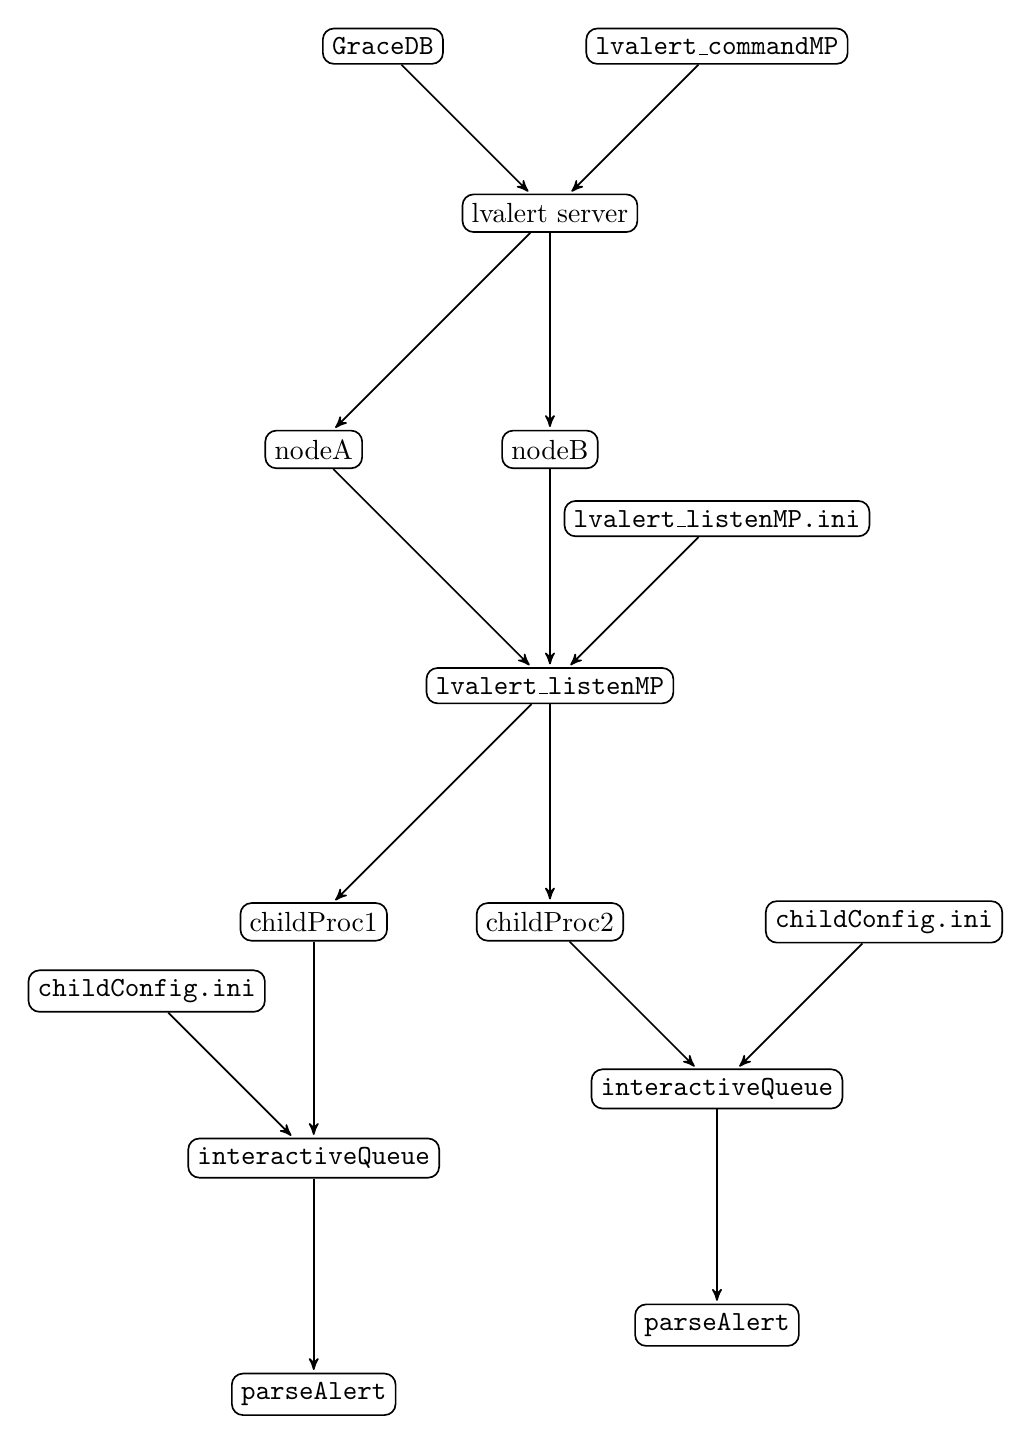
\begin{tikzpicture}[->,>=stealth', shorten >= 1pt, auto, node distance=3.00cm, semithick]
        \tikzset{
           server/.style={
                        rectangle,
                        rounded corners,
                        draw=black,
                        fill=none,
                        text=black
                       },
           lvalertNode/.style={
                        rectangle,
                        rounded corners,
                        draw=black,
                        fill=none,
                        text=black
                       },
           mpPipe/.style={
                        rectangle,
                        rounded corners,
                        draw=black,
                        fill=none,
                        text=black
                       },
           lvalertMP/.style={
                        rectangle,
                        rounded corners,
                        draw=black,
                        fill=none,
                        text=black
                       },
           config/.style={
                        rectangle,
                        rounded corners,
                        draw=black,
                        fill=none,
                        text=black
                       },
           childProc/.style={
                        rectangle,
                        rounded corners,
                        draw=black,
                        fill=none,
                        text=black
                       },
                 };
    %--------------------
        \node[server]      (lvalertServer)                                {lvalert server};

        \node[server]      (GraceDB)       [above left of=lvalertServer]  {\GraceDB};
        \node[lvalertMP]   (lvalertCmd)    [above right of=lvalertServer] {\lvalertCommandMP};

        \node[lvalertNode] (nodeB)         [below of=lvalertServer]       {nodeB};
        \node[lvalertNode] (nodeA)         [left of=nodeB]  {nodeA};

        \node[lvalertMP]   (lvalertMP)     [below of=nodeB]               {\lvalertListenMP};
        \node[config]      (lvalertConfig) [above right of=lvalertMP]               {\lvalertMPini};

        \node[childProc]   (childProc2)    [below of=lvalertMP]           {childProc2};
        \node[childProc]   (childProc1)    [left of=childProc2]           {childProc1};

        \node[childProc]   (intractvQ1)    [below of=childProc1]          {\interactiveQueue};
        \node[childProc]   (intractvQ2)    [below right of=childProc2]    {\interactiveQueue};

        \node[config]      (childConfig1)  [above left of=intractvQ1]     {\childConfigini};
        \node[config]      (childConfig2)  [above right of=intractvQ2]    {\childConfigini};

        \node[childProc]   (parseAlert1)   [below of=intractvQ1]          {\parseAlert};
        \node[childProc]   (parseAlert2)   [below of=intractvQ2]          {\parseAlert};
    %--------------------
        \path (GraceDB)       edge (lvalertServer)
              (lvalertCmd)    edge (lvalertServer)

              (lvalertServer) edge (nodeA)
              (lvalertServer) edge (nodeB)
%              (lvalertServer) edge (nodeC)

              (nodeA)         edge (lvalertMP)
              (nodeB)         edge (lvalertMP)
%              (nodeC)         edge (lvalertMP)

              (lvalertConfig) edge (lvalertMP)

              (lvalertMP)     edge (childProc1)
              (lvalertMP)     edge (childProc2)

              (childConfig1)  edge (intractvQ1)
              (childConfig2)  edge (intractvQ2)

              (intractvQ1)    edge (parseAlert1)
              (intractvQ2)    edge (parseAlert2)

              (childProc1)    edge (intractvQ1)
              (childProc2)    edge (intractvQ2);
    \end{tikzpicture}
    \end{center}
    \caption{The flow of \alert messages between processes.}
    \label{fig: alert flow}
\end{figure}

%-------------

\subsection{workflow within \interactiveQueue}
\label{sec: interactiveQueue workflow}

\interactiveQueue~is actually quite minimalistic in it's function. 
It begins by instantiating all the required data structures and loading the appropriate libraries (determined by the \texttt{process\_type} option in \childConfigini).
Then it enters a persistent loop.
During each epoch of the loop it
\begin{enumerate}
    \item{checks whether there is a new alert message in the \multiprocessingConnection~object's buffer
        \begin{itemize}
            \item{if so, it reads in the alert (and \texttt{t0}) and delegates the interpretation to \parseAlert.}
        \end{itemize}
         }
    \item{checks to see if the first item in the \SortedQueue~has expired
        \begin{itemize}
            \item{while the first item in \textit{queue} is expired, execute it iteratively}
            \item{execution is achieved through delegation to \QueueItem.execute, which in turn delegates to \Task.execute and updates the \QueueItem's attributes accordingly.}
        \end{itemize}
         }
    \item{cleans up the data structures
        \begin{itemize}
            \item{removes any keys from \textit{queueByGraceID} that correspond to empty \SortedQueue}
            \item{if there are too many \textit{complete} \QueueItem~instances in \textit{queue}, clean it up with a call to \SortedQueue.clean}
        \end{itemize}
         }
    \item{if necessary, wait a bit before proceeding to the next epoch. This is controlled by the \textit{sleep} option to \interactiveQueue.}
\end{enumerate}
Figure \ref{fig: interactiveQueue} demonstartes this pictorially.

\begin{figure}

    \begin{center}
    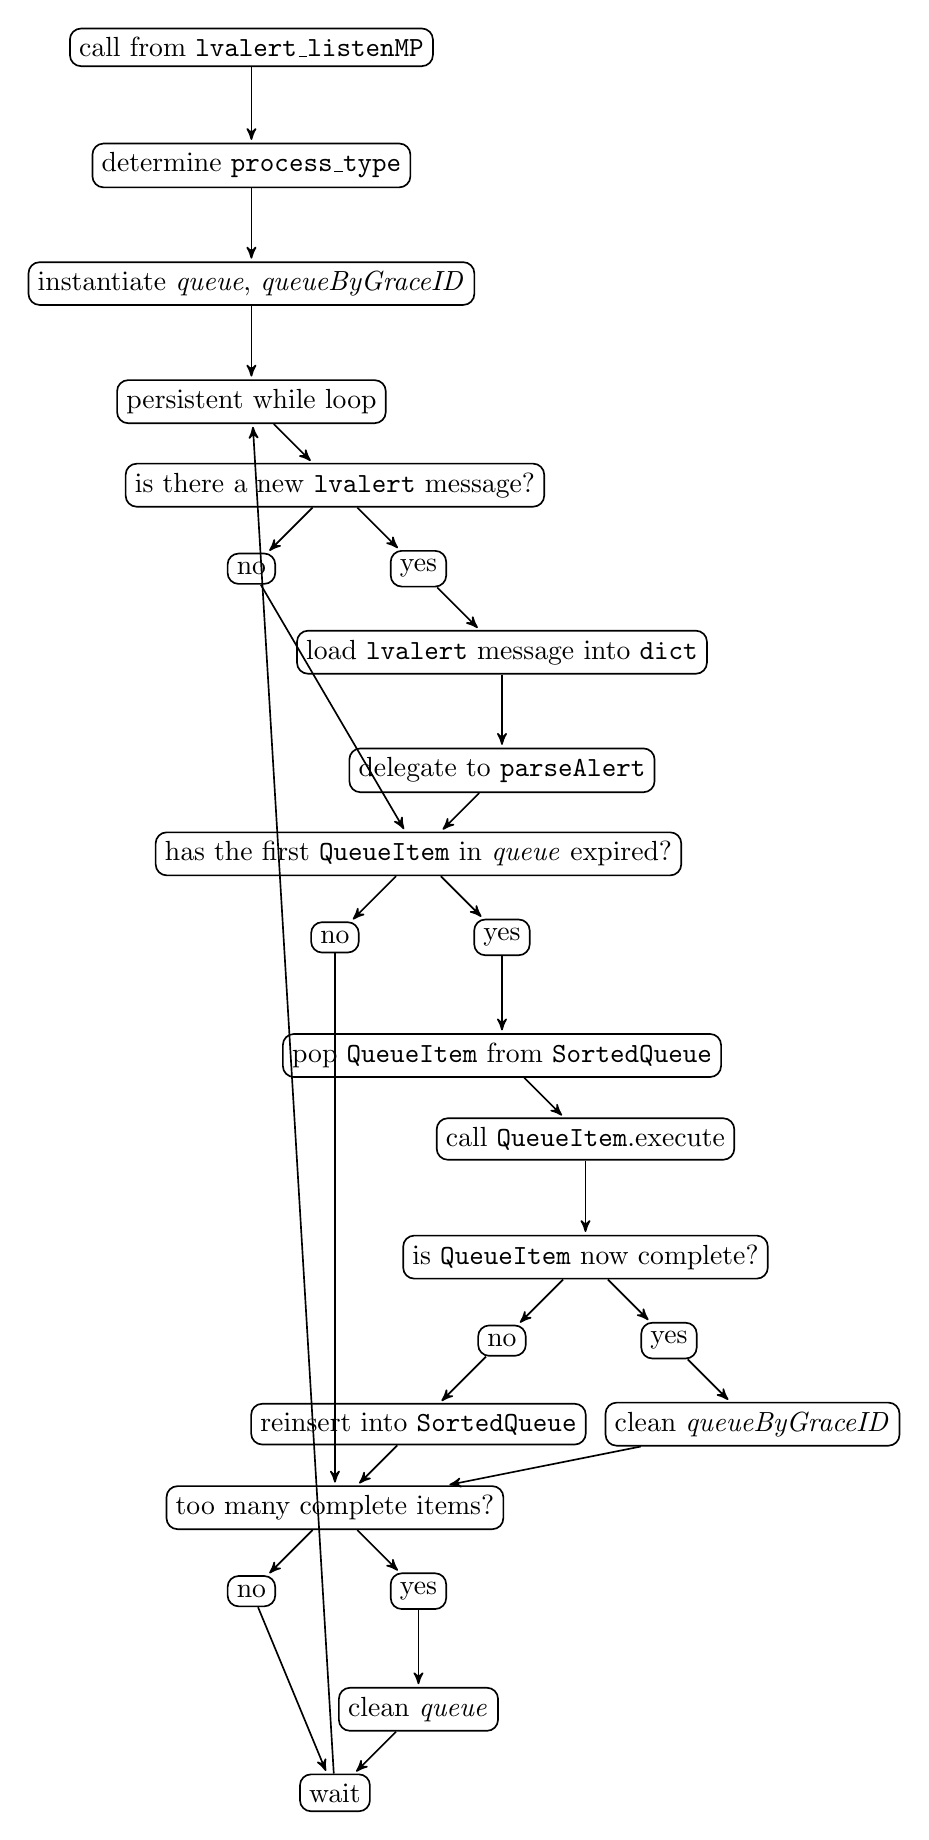
\begin{tikzpicture}[->,>=stealth', shorten >= 1pt, auto, node distance=1.50cm, semithick]
        \tikzset{
           node/.style={
                        rectangle,
                        rounded corners,
                        draw=black,
                        fill=none,
                        text=black
                       },
                 };
    %--------------------
        \node[node]      (call)                            {call from \lvalertListenMP};
        \node[node]      (procType) [below of=call]        {determine \texttt{process\_type}};
        \node[node]      (instantiate) [below of=procType] {instantiate \textit{queue}, \textit{queueByGraceID}};

        \node[node]      (while) [below of=instantiate]    {persistent while loop};

        \node[node]      (newAlert) [below right of=while] {is there a new \alert~message?};

          \node[node]      (newAlertYes) [below right of=newAlert] {yes};
            \node[node]      (loadAlert)   [below right of=newAlertYes] {load \alert~message into \pythondict};
            \node[node]      (parseAlert)  [below of=loadAlert] {delegate to \parseAlert};
        
          \node[node]      (newAlertNo)  [below left of=newAlert]  {no};

        \node[node]      (hasExpired)  [below left of=parseAlert] {has the first \QueueItem~in \textit{queue} expired?};

          \node[node]      (hasExpiredYes) [below right of=hasExpired] {yes};
            \node[node]    (pop) [below of=hasExpiredYes] {pop \QueueItem~from \SortedQueue};
            \node[node]      (itemExecute) [below right of=pop] {call \QueueItem.execute};
            \node[node]      (itemComplete) [below of=itemExecute] {is \QueueItem~now complete?};
              \node[node]      (itemCompleteYes) [below right of=itemComplete] {yes};
                \node[node] (popGID) [below right of=itemCompleteYes] {clean \textit{queueByGraceID}};
              \node[node]      (itemCompleteNo)  [below left of=itemComplete] {no};
                \node[node] (reinsert) [below left of=itemCompleteNo] {reinsert into \SortedQueue};
          \node[node]      (hasExpiredNo) [below left of=hasExpired] {no};
        \node[node] (2many) [below left of=reinsert] {too many complete items?};
          \node[node] (2manyYes) [below right of=2many] {yes};
            \node[node] (clean) [below of=2manyYes] {clean \textit{queue}};
          \node[node] (2manyNo) [below left of=2many] {no};
        \node[node] (wait) [below left of=clean] {wait};
    %--------------------
        \path (call)        edge (procType)
              (procType)    edge (instantiate)
              (instantiate) edge (while)
              (while)       edge (newAlert)
              (newAlert)    edge (newAlertYes)
              (newAlert)    edge (newAlertNo)
              (newAlertYes) edge (loadAlert)
              (loadAlert)   edge (parseAlert)
              (parseAlert)  edge (hasExpired)
              (newAlertNo)  edge (hasExpired)
              (hasExpired)  edge (hasExpiredYes)
              (hasExpired)  edge (hasExpiredNo)
              (hasExpiredYes) edge (pop)
              (pop)         edge (itemExecute)
              (itemExecute) edge (itemComplete)
              (itemComplete) edge (itemCompleteYes)
              (itemComplete) edge (itemCompleteNo)
              (itemCompleteYes) edge (popGID)
              (itemCompleteNo) edge (reinsert)
              (hasExpiredNo) edge (2many)
              (reinsert) edge (2many)
              (popGID) edge (2many) 
              (2many) edge (2manyYes)
              (2many) edge (2manyNo)
              (2manyYes) edge (clean)
              (2manyNo) edge (wait)
              (clean) edge (wait)
              (wait) edge (while)
        ;
    \end{tikzpicture}
    \end{center}
    \caption{work flow within \interactiveQueue}
    \label{fig: interactiveQueue}
\end{figure}

%-------------

\subsection{example workflow within \parseAlert}
\label{sec: parseAlert workflow}

\parseAlert's actual workings should be defined in extensions of \lvalertMP.
However, we provide a suggested roadmap in Figure \ref{fig: parseAlert}.
It is important to remember that \parseAlert~\textit{must} return the change in the number of completed \QueueItem~instances within \textit{queue}.
If it does not do this correctly, then \interactiveQueue~will not clean up \textit{queue} correctly.

\begin{figure}

    \begin{center}
    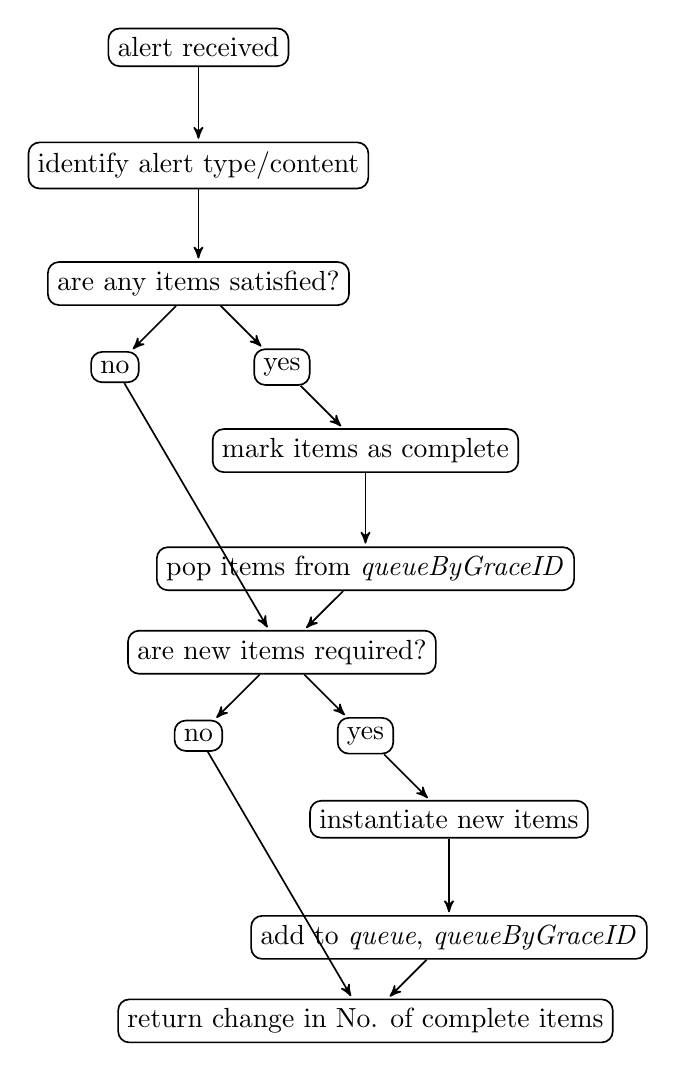
\begin{tikzpicture}[->,>=stealth', shorten >= 1pt, auto, node distance=1.50cm, semithick]
        \tikzset{
           node/.style={
                        rectangle,
                        rounded corners,
                        draw=black,
                        fill=none,
                        text=black
                       },
                 };
        %----------------
        \node[node] (alert) {alert received};
        \node[node] (identify) [below of=alert] {identify alert type/content};
        \node[node] (complete) [below of=identify] {are any items satisfied?};
          \node[node] (completeYes) [below right of=complete] {yes};
            \node[node] (mark) [below right of=completeYes] {mark items as complete};
            \node[node] (popGID) [below of=mark] {pop items from \textit{queueByGraceID}}; 
          \node[node] (completeNo)  [below left of=complete] {no};
        \node[node] (new) [below left of=popGID] {are new items required?};
          \node[node] (newYes) [below right of=new] {yes};
            \node[node] (instantiate) [below right of=newYes] {instantiate new items};
            \node[node] (insert) [below of=instantiate] {add to \textit{queue}, \textit{queueByGraceID}};
          \node[node] (newNo) [below left of=new] {no};
        \node[node] (return) [below left of=insert] {return change in No. of complete items};
        %----------------
        \path (alert) edge (identify)
              (identify) edge (complete)
              (complete) edge (completeYes)
              (complete) edge (completeNo)
              (completeYes) edge (mark)
              (mark) edge (popGID)
              (popGID) edge (new)
              (completeNo) edge (new)
              (new) edge (newNo)
              (new) edge (newYes)
              (newYes) edge (instantiate)
              (instantiate) edge (insert)
              (insert) edge (return)
              (newNo) edge (return)
        ;
    \end{tikzpicture}
    \end{center}
    \caption{figure showing what happens within \parseAlert~as it is written within \eventSupervisor}
    \label{fig: parseAlert}
\end{figure}

For a concrete example of how \eventSupervisor~implements \parseAlert~functionality, we refer to \S\ref{sec: eventSupervisor parseAlert}.

%------------------------

\newpage

\FIXME{left off here!}

\newpage

\section{suggested extensions}
\label{sec: suggested extensions}

%-------------

\subsection{\eventSupervisor \Task extension}
\label{sec: eventSupervisor Task}

\FIXME{walk through how \eventSupervisor~extends \Task~object to send emails as part of the the execute method, etc.}

%-------------

\subsection{\eventSupervisor \QueueItem extension}
\label{sec: eventSupervisor QueueItem}

\FIXME{walk through the extension to \QueueItem~within \eventSupervisor~so that it passes the necessary things to the \Task~extension}
\FIXME{may also need to change QI.execute() signature within \eventSupervisor~so that it passes GID, gdb $\rightarrow$ Task.execute correctly (from attributes rather than input arguments)}

%-------------

\subsection{\eventSupervisor \parseAlert}
\label{sec: eventSupervisor parseAlert}

\FIXME{walk through \eventSupervisor~\parseAlert~and how it standardizes \_\_init\_\_ API and the relation to sub-modules and config files.}

%-------------

\subsection{\eventSupervisor \texttt{bayestar} example}
\label{sec: eventSupervisor bayestar}

\FIXME{walk through the \texttt{bayestar} module within \eventSupervisor~to demonstrate class extensions for ``well behaved'' follow-up processes.}

%-------------

\subsection{possible implementations for \approvalProcessor}
\label{sec: approvalProcessor}

\FIXME{a suggestion of how \approvalProcessor~might accomplish it's goals using the \SortedQueue~architecture. Essentially, this becomes a scheduler (like Condor's queue) but with limited scope and functionality.}

%-------------------------------------------------
\end{document}
%-------------------------------------------------
